%Modelo da Dissertação de Mestrado da EN
% TMDEI Thesis EN Style
% 
% Based on MastersDoctoralThesis Version 1.2 by Vel (vel@latextemplates.com) and
% Johannes Böttcher, downloaded from (21/11/15):
% http://www.LaTeXTemplates.com
%
% Authors:
%  Vel (vel@ latextemplates. com)
%  Johannes Böttcher%
%
% Adapted to Thesis EN Style (JUL/2019) by 
%  HILÁRIO ARAÚJO (rocha.araujo@marinha.pt) 
%
%%%%%%%%%%%%%%%%%%%%%%%%%%%%%%%%%%%%%%%%%

%-----------------------------------------%
%--------CONFIGURAÇÃO INICIAL-------------%
%-----------------------------------------%

\documentclass[12pt, % O tamanho da fonte do documento padrão, opções: 10pt, 11pt, 12pt
%oneside, % Dois lados (margens alternadas) para ligação por padrão, uncomment a mudar para um lado (para fins de desenho / leitura)
portuguese, %portuguese,% for Portuguese; english for English; delete temporary files if you change language (e.g. 'make clean; make')
singlespacing, % Espaçamento de linha única, alternativas: onehalfspacing or doublespacing (para fins de redação / leitura)
%draft, % Uncomment para ativar o modo de rascunho (sem imagens, sem links, caixas de texto overfull indicadas)
%nolistspacing, % Se o documento for de meio-espaço ou de espaçamento duplo, uncomment para definir o espaçamento nas listas como único
%liststotoc, % Uncomment para adicionar a lista de figuras / tabelas / etc ao índice (não recomendado)
%toctotoc, % Uncomment para adicionar o índice principal ao índice (não recomendado)
parskip, % Adicione espaço entre parágrafos (recomendado)
%nohyperref, % Uncomment para não carregar o pacote hyperref (não recomendado)
nohyperreflinkcolor, % links de hyperref não são coloridos (comment para links de cores, por exemplo, para produzir uma versão somente eletrônica)
headsepline, % Uncomment para obter uma linha sob o cabeçalho
]{tmdei-style} % O arquivo de classe que especifica a estrutura do documento



\usepackage{tikz} % Required for creating graphics programmatically (can be removed if not used)
%\usetikzlibrary{arrows} % Required for fancy arrows in TiKZ graphics (can be removed if not used)

\usepackage{pgfplots} % Required for drawing high--quality function plots (can be removed if not used)
\pgfplotsset{compat=newest}

% Next you have examples of admissable citation styles; we recomend using the authoryear-comp citation style (which resembles Harvard); don't forget to only uncomment one
%
% authoryear-comp: recommended citation style (e.g. (Buendía, 1860), (Buendía 1910, Arcadio 1940))
\usepackage[style=authoryear-comp,backend=biber]{biblatex} % Bibtex backend with the authoryear-comp citation style (authoryear citations, bibliography ordered alphabetically)

% numeric citation style (e.g. [1], [1-3])
%\usepackage[style=numeric-comp,sorting=none,backend=biber]{biblatex} % Bibtex backend with the numeric-comp citation style (numeric citations, bibliography ordered by appearance)

% alphabetic citation style (e.g. [Buendía10], [Buendía10, Arcadio40])
%\usepackage[style=alphabetic,sorting=none,backend=biber]{biblatex} % Bibtex backend with the alphabetic citation style (alphabetic citations, bibliography ordered by appearance)

\addbibresource{mainbibliography.bib} % O nome da base de dados da sua bibliografia

\makeglossaries % cria o glossário.



%-----------------------------------------%
%--------INFORMAÇÃO SOBRE A TESE-------------%
%-----------------------------------------%
\thesistitle{{[}Título Principal {]}} %Escreva o título da tese, pode referenciar o titulo ao longa da dissertação utilizando o comando (\ttitle)

\thesissubtitle{{[}Subtítulo da Tese{]}} %Escreva o subtítulo da tese, pode referenciar o titulo ao longa da dissertação utilizando o comando (\subttitle)

\author{Nome do Orientando} % Escreva o seu nome, pode referenciar o autor ao longa da dissertação utilizando o comando (\authorname)

\thesisdate{Escola Naval, \today} % data da impressão da tese, pode referenciar a data ao longa da dissertação utilizando o comando (\tdate)

\subjectarea{Engenharia Naval Ramo de Armas e Eletrónica} % Especializa a tua especialidade: Engenharia Naval Ramo de Armas e Eletrónica, Engenharia Naval Ramo de Mecânica, Marinha, Fuzileiros, Marinha e Administração Naval
%poderá referenciar-lo ao longo do seu trabalho com o comando (\areaname)

\supervisor{Nome do \textsc{Orientador}} % O nome do seu supervisor, isto é usado na página da contra capa,  poderá referenciar-lo ao longo do seu trabalho com o comando (\supname)

%\cosupervisor{Dr. Jack \textsc{Smith}} % O nome do seu co-orientador, isto é usado na página da contra capa,  poderá referenciar-lo ao longo do seu trabalho com o comando (\cosupname) (comenta, se não tiveres co-orientador)


\keywords{Keyword1, ..., Keyword6} % Defina até 6 palavras-chave que descrevam melhor o seu trabalho, e poderá referenciar-las ao longo do seu trabalho com o comando (\keywordnames)


\hypersetup{pdftitle=\ttitle} % Set the PDF's title to your title
\hypersetup{pdfauthor=\authorname} % Set the PDF's author to your name
\hypersetup{pdfkeywords=\keywordnames} % Set the PDF's keywords to your keywords


\begin{document}


%-----------------------------------------%
%--------PÁGINAS INICIAIS-------------%
%-----------------------------------------%

% Inclui as páginas iniciais da sua tese
%O frontmmatter são as chamadas páginas iniciais, terá de atualizar as respetivas secções.

%-----------------------------------------%
%    CONFIGURAÇÃO INICIAL                 %
%-----------------------------------------%

%Todos os acrônimos devem ser escritos neste arquivo.

\newacronym{RTS}{RTS}{Real-Time System}
\newacronym{GPOS}{GPOS}{General Purpose Operating System}
\newacronym{RTOS}{RTOS}{Real-Time Operating System}
\newacronym{PGF}{PGF}{Portable Graphics Format}


\frontmatter % Use roman page numbering style (i, ii, iii, iv...) for the pre-content pages

\pagestyle{plain} % Default to the plain heading style until the thesis style is called for the body content

%----------------------------------------------------------------------------------------
%	CAPA
%----------------------------------------------------------------------------------------
\maketitlepage


%----------------------------------------------------------------------------------------
%	CONTRA CAPA
%----------------------------------------------------------------------------------------
\makeconttitlepage


%-----------------------------------------%
%      EPÍGRAFE     (opcional)                     
%-----------------------------------------%
\begin{epigraph}
\null \vfill
\begin{flushright}

A epígrafe traduz-se pela inscrição de sentença conceituosa que, de algum modo inspirou o autor na elaboração do trabalho ou nas suas ações correntes, e que o mesmo considere importante revelar no trabalho. Tem uma natureza facultativa.

\end{flushright}
\vfill \null%
\end{epigraph}%



%----------------------------------------------------------------------------------------
%	DEDICATÓRIA  (opcional)
%----------------------------------------------------------------------------------------
%\dedicatory{For/Dedicated to/To my\ldots}
\begin{dedicatory}
\null \vfill
\begin{flushright}

A dedicatória tem por finalidade prestar homenagem ou dedicar o trabalho a alguém próximo ou que tenha um especial significado para o autor do trabalho. 

É, também, um elemento facultativo na estrutura do trabalho, mas é usual que seja feita dedicando o trabalho aos pais, à família mais chegada ou a alguém com relevância especial na vida do autor. 

\end{flushright}
\vfill \null%
\end{dedicatory}


%----------------------------------------------------------------------------------------
%	AGRADECIMENTOS (opcional)
%----------------------------------------------------------------------------------------

\begin{acknowledgements}

Agradecimento é a expressão registada de uma gratidão às pessoas, entidades ou instituições que, de algum modo, contribuíram para a elaboração do trabalho. Sendo um elemento opcional, quando exista deve incluir-se na frente de folha a colocar logo após a folha de rosto ou das folhas da epígrafe e/ou da dedicatória, deixando o verso em branco.

\end{acknowledgements}




%----------------------------------------------------------------------------------------
%	RESUMO
%----------------------------------------------------------------------------------------

\begin{abstract}

\noindent \textbf{\ Subtítulo caso queira!}

Segue-se, com caráter obrigatório, um resumo em língua portuguesa e em língua inglesa (abstract), cada um deles com um máximo de 300 palavras.

Após cada um dos resumos devem ser indicadas cinco palavras-chave – português e inglês – para indexação futura.

% As palavras chave terão de ser definidas no ficheiro main.tex depois da linha de código keywords
\end{abstract}


%----------------------------------------------------------------------------------------
%	ABSTRACT 
%----------------------------------------------------------------------------------------
\begin{abstractotherlanguage}
% here you put the abstract in the "other language": English, if the work is written in Portuguese; Portuguese, if the work is written in English.


\noindent \textbf{\ Subtitle if you want}
\noindent 

Trabalhos escritos em língua Inglesa devem incluir um resumo alargado com cerca de 1000 palavras, ou duas páginas.

Se o trabalho estivesse escrito em Português, este resumo seria em língua Inglesa, com cerca de 200 palavras, ou uma página.

Para alterar a língua basta ir às configurações do documento no ficheiro \file{main.tex} e alterar para a língua desejada ('english' ou 'portuguese')\footnote{Alterar a língua requer apagar alguns ficheiros temporários; O target \keyword{clean} do \keyword{Makefile} incluído pode ser utilizado para este propósito.}. Isto fará com que os cabeçalhos incluídos no template sejam traduzidos para a respetiva língua.

\noindent \newline \textbf{Key words: } \text{keyword1, ..., keyword2}
\end{abstractotherlanguage}



%----------------------------------------------------------------------------------------
%	ÍNDICE DE CONTEÚDO / FIGURAS / TABELAS
%----------------------------------------------------------------------------------------

\tableofcontents % Imprime o índice principal

\listoffigures % Imprime a lista de figuras

\listoftables % Imprime a lista de tabelas

\iflanguage{portuguese}{
\renewcommand{\listalgorithmname}{Lista de Algor\'itmos}
}
\listofalgorithms % Prints the list of algorithms
%\addchaptertocentry{\listalgorithmname} %Uncomment para mostrar no índice a lista de algoritmos


\renewcommand{\lstlistlistingname}{List of Source Code}
\iflanguage{portuguese}{
\renewcommand{\lstlistlistingname}{Lista de C\'odigo}
}
\lstlistoflistings % Imprime a lista de listagens (código-fonte da linguagem de programação)

%\addchaptertocentry{\lstlistlistingname} %Uncomment para mostrar a lista de de código no índice


%----------------------------------------------------------------------------------------
%	ABREVIATURAS
%----------------------------------------------------------------------------------------
%\begin{abbreviations}{ll} % IncluI uma lista de abreviações (uma tabela de duas colunas)
%%\textbf{LAH} & \textbf{L}ist \textbf{A}bbreviations \textbf{H}ere\\
%%\textbf{WSF} & \textbf{W}hat (it) \textbf{S}tands \textbf{F}or\\
%\end{abbreviations}

%----------------------------------------------------------------------------------------
%	SÍMBOLOS
%----------------------------------------------------------------------------------------

\begin{symbols}{lll} % Inclui uma lista de símbolos (uma tabela de três colunas)

$a$ & distance & \si{\meter} \\
$P$ & power & \si{\watt} (\si{\joule\per\second}) \\
%%Símbolo, nome e unidade

\addlinespace % espaçamento para separar os símbolos romanos dos grego

$\omega$ & angular frequency & \si{\radian} \\

\end{symbols}



%----------------------------------------------------------------------------------------
%	ACRÓNIMOS
%----------------------------------------------------------------------------------------

\newcommand{\listacronymname}{List of Acronyms}
\iflanguage{portuguese}{
\renewcommand{\listacronymname}{Lista de Acr\'onimos}
}

%Use GLS
\glsresetall
\printglossary[title=\listacronymname,type=\acronymtype,style=long]


%----------------------------------------------------------------------------------------
%	ACABOU - BOM TRABALHO
%----------------------------------------------------------------------------------------

\mainmatter % Começar numeração da página com numéros árabes (1,2,3 ...)
\pagestyle{thesis} % Colocar os cabeçalhos nas páginas com o estilo definido para o corpo da tese



%-----------------------------------------%
%--------CAPÍTULOS-------------%
%-----------------------------------------%

% Inclui os capítulos da tese como das respetivas pastas separadas por cada capítulo

% Capítulo 1
% 
\chapter{Estrutura da Dissertação de Mestrado} % Título do capítulo
\label{chap:Chapter1} % Para fazer referência a esta secção ao longo da dissertação, use o comando Chapter~\ref{Chapter1}


%-------------------------------------------------------------------------------
%---------
%
\section{Introdução} 
\label{sec:chap1_introduction} %Para fazer referência a esta secção ao longo da dissertação, use o comando Section~\ref{sec:chap1_introduction}

A introdução prepara o leitor para uma leitura organizada e uma melhor compreensão do trabalho científico que se está a apresentar. Deve por isso começar por apresentar, de forma breve, a problemática em que se insere o trabalho científico.
Sempre que for necessário fazer este enquadramento de forma detalhada e mais longa, deve apenas referir-se o assunto na introdução indicando que a apresentação mais detalhada será feita num dos primeiros capítulos (normalmente o primeiro).\\ Feita, contudo, esta apresentação do assunto, expondo a problemática subjacente ao mesmo, deve apresentar-se o problema, ou problemas, objeto do estudo efetuado, a que se segue uma explicação das vias seguidas na investigação e da forma como elas transparecem na estrutura adotada para a apresentação. Seguem-se, se forem relevantes e necessárias, algumas explicações sobre a metodologia do trabalho, terminando com os objetivos que se pretende alcançar. Sempre que for necessário, para uma melhor compreensão por parte do leitor, pode dividir-se a introdução em pequenos subcapítulos, indicando objetivos, vias seguidas na investigação, metodologias e resultados pretendidos.//
Este capítulo não tem numeração específica e deve iniciar-se ao cimo de uma página ímpar (à direita), independentemente do facto da página anterior ser deixada com verso em branco. 



\section{Capítulos}

Segue-se o corpo principal do trabalho, dividido em capítulos, numerados em numeração árabe (1, 2, 3,...), que podem subdividir-se em subcapítulos, sucessivamente, igualmente numerados segundo a lógica

1. Capítulo 

1.1 Subcapítulo 

1.1.1 Sub-subcapítulo 

etc...

Aos capítulos e subcapítulos devem ser dados títulos, em letra destacada em negrito, de corpo sucessivamente 14, 13 e 12, sempre encostados à margem esquerda da página sem qualquer avanço.

Não é possível apresentar um critério único para o ordenamento de capítulos e subcapítulos, decorrendo esta estrutura da natureza do próprio trabalho, variando consoante a área disciplinar ou científica do mesmo e das suas características próprias.\\
Nalguns casos terá uma natureza explicativa, noutros passará pela exposição de resultados e sua interpretação, envolvendo a apresentação de critérios, tabelas de resultados, memória descritiva, etc.

Cada um dos capítulos deve começar ao cimo de uma página ímpar (à direita).

\section{Conclusão}
A conclusão segue-se ao corpo principal dos capítulos que constituem o trabalho, realçando, de forma resumida e nos aspetos mais relevantes, os passos seguidos e os resultados obtidos (mas evitando fazer um resumo que repita aspetos do corpo). Devem expor-se as dificuldades e limitações sentidas, sobretudo se as mesmas limitaram a investigação e prejudicaram o alcançar dos resultados propostos na introdução. E, de igual modo, se a investigação desenvolvida mostrou novas vias de trabalho que não puderam ser desenvolvidas, devem evidenciar-se os caminhos que foram abertos, avançando com sugestões e propostas para trabalhos futuros que deem continuidade ao projeto presente.

Este capítulo não deve ser numerado, devendo começar ao início de uma página Ímpar (à direita), mesmo que a página anterior se encontre em branco.
% Chapter 2

\chapter{About \LaTeX{} and How to Use This Template} % Main chapter title

\label{chap:Chapter2} % For referencing the chapter elsewhere, use \ref{chap:Chapter2} 

%----------------------------------------------------------------------------------------

\section{Learning \LaTeX{}}

\LaTeX{} is not a \textsc{wysiwyg} (What You See is What You Get) program, unlike word processors such as Microsoft Word or Apple's Pages. Instead, a document written for \LaTeX{} is actually a simple, plain text file that contains \emph{no formatting}. You tell \LaTeX{} how you want the formatting in the finished document by writing in simple commands amongst the text, for example, if I want to use \emph{italic text for emphasis}, I write the \verb|\emph{text}| command and put the text I want in italics in between the curly braces. This means that \LaTeX{} is a \enquote{mark-up} language, very much like HTML.

\subsection{A (not so short) Introduction to \LaTeX{}}

If you are new to \LaTeX{}, there is a very good eBook -- freely available online as a PDF file -- called, \enquote{The Not So Short Introduction to \LaTeX{}}. The book's title is typically shortened to just \emph{lshort}. You can download the latest version (as it is occasionally updated) from here:
\url{http://www.ctan.org/tex-archive/info/lshort/english/lshort.pdf}

It is also available in several other languages. Find yours from the list on this page: \url{http://www.ctan.org/tex-archive/info/lshort/}

It is recommended to take a little time out to learn how to use \LaTeX{} by creating several, small `test' documents, or having a close look at several templates on:\\ 
\url{http://www.LaTeXTemplates.com}\\ 
Making the effort now means you're not stuck learning the system when what you \emph{really} need to be doing is writing your thesis.

\subsection{A Short Math Guide for \LaTeX{}}

If your thesis is going to contain heavy mathematical content, be sure that \LaTeX{} will make it look beautiful, even though it won't be able to solve the equations for you.

The \enquote{Not So Short Introduction to \LaTeX} (available on \url{http://www.ctan.org/tex-archive/info/lshort/english/lshort.pdf}{CTAN}) should tell you everything you need to know for most cases of typesetting mathematics. If you need more information, a much more thorough mathematical guide is available from the AMS called, \enquote{A Short Math Guide to \LaTeX} and can be downloaded from:
\url{ftp://ftp.ams.org/pub/tex/doc/amsmath/short-math-guide.pdf}

There are many different \LaTeX{} symbols to remember, luckily you can find the most common symbols in \url{http://ctan.org/pkg/comprehensive}{The Comprehensive \LaTeX~Symbol List}.

You can write an equation, which is automatically given an equation number by \LaTeX{} like this:
\begin{verbatim}
\begin{equation}
E = mc^{2}
\label{eqn:Einstein}
\end{equation}
\end{verbatim}

This will produce Einstein's famous energy-matter equivalence equation:
\begin{equation}
E = mc^{2}
\label{eqn:Einstein}
\end{equation}

All equations you write (which are not in the middle of paragraph text) are automatically given equation numbers by \LaTeX{}. If you don't want a particular equation numbered, use the unnumbered form:
\begin{verbatim}
\[ a^{2}=4 \]
\end{verbatim}

\LaTeX{} automatically adjusts the style of the math expressions according to the case if they are inline or not (so that they occupy more or less space), but you can set this explicitly. For instance, if you want an in-line mathematical element to display as a equation-like element put \verb|\displaystyle| before that element. Use \verb|\textstyle| for small, inline-like maths, before the command that generates the element.

\subsection{Obtaining \LaTeX{}}
 
The \LaTeX{} distribution is available for many systems including Windows, Linux and Mac OS X. Check the webpage for the \LaTeX{} project for more information: \url{https://latex-project.org/ftp.html}.

%----------------------------------------------------------------------------------------

\section{Getting Started with this Template}

If you are familiar with \LaTeX{}, then you should explore the directory structure of the template and then proceed to place your own information into the \emph{THESIS INFORMATION} block of the \file{main.tex} file. You can then modify the rest of this file to your unique specifications. Section \ref{FillingFile} on page \pageref{FillingFile} will help you do this. Make sure you also read section \ref{ThesisConventions} about thesis conventions to get the most out of this template.

If you are new to \LaTeX{} it is recommended that you carry on reading through the rest of the information in this document.

\subsection{About this Template}

This \LaTeX{} Thesis Template is originally based and created around a \LaTeX{} style file created by Steve R.\ Gunn from the University of Southampton (UK), department of Electronics and Computer Science. You can find his original thesis style file at his site, here:
\url{http://www.ecs.soton.ac.uk/~srg/softwaretools/document/templates/}

Steve's \file{ecsthesis.cls} was then taken by Sunil Patel who modified it by creating a skeleton framework and folder structure to place the thesis files in. The resulting template can be found on Sunil's site here:
\url{http://www.sunilpatel.co.uk/thesis-template}

Sunil's template was made available through \url{http://www.LaTeXTemplates.com} where it was modified many times based on user requests and questions. Version 2.0 and onwards of this template represents a major modification to Sunil's template and is, in fact, hardly recognisable. The work to make version 2.0 possible was carried out by \url{mailto:vel@latextemplates.com} {Vel} and Johannes Böttcher.

Vel's and Böttcher template was adapted to fit the TMDEI/ISEP dissertation formatting specifications. This adaptation was done by Nuno Pereira (nap@isep.ipp.pt) and Paulo Baltarejo (pbs@isep.ipp.pt) in December 2015. It was also based on the specifications earlier defined by Fátima Rodrigues (mfc@isep.ipp.pt).
%----------------------------------------------------------------------------------------

\section{What this Template Includes}

\subsection{Folders}

This template is composed of several files and folders. The folder names are mostly self-explanatory:

\keyword{frontmatter} -- this is the folder holding the \file{frontmatter.tex} where are defined the dedicatory, abstract, acknowledgement, contents pages, list of figures, tables and others.

\keyword{CH1, CH2, ...} -- these are the folders where you put the contents of each chapter. Each chapter should go in its own separate folder. Inside each chapter folder there is one (or more) \keyword{.tex} with the contents of the chapter, and an \keyword{assets} folder which contains the figures and other graphical elements of the chapter (such as algorithms, source code, plots, ...).

\keyword{appendices} -- this is the folder where you put the appendices. Each appendix should go into its own separate \file{.tex} file. An example and template are included in the directory.

\keyword{build} -- this is the folder where the output of building your document is put. Everytime you build your document,
 \LaTeX{} creates a number of auxiliary files that are written to this folder. These auxiliary files can be ignored or deleted as \LaTeX{} and BibTeX will regenerate them\footnote{Some changes require rebuilding temporary files again; actually, a document with citations may require up to three passes. For this reason, we recommend using the included \keyword{Makefile} which deals with such details}. Note that the resulting \file{pdf} file is written to this folder and then copied to the root folder of the template.

\subsection{Files}

Included are also several files, most of them are plain text and you can see their contents in a text editor. After initial compilation, you will see that more auxiliary files are created by \LaTeX{} or BibTeX and which you don't need to delete or worry about\footnote{Note that some changes (such as changing the language of the template require deleting some of these temporary files) the included \keyword{Makefile} has a \keyword{clean} rule to do this automatically}:

\keyword{main-bibliography.bib} -- this is an important file that contains all the bibliographic information and references that you will be citing in the thesis for use with BibTeX. You can write it manually, but there are reference manager programs available that will create and manage it for you. Bibliographies in \LaTeX{} are a large subject and you may need to read about BibTeX before starting with this (check, for example: \url{http://www.bibtex.org/Using/}). Many modern reference managers will allow you to export your references in BibTeX format which greatly eases the amount of work you have to do.

\keyword{tmdei-style.cls} -- this is an important file. It is the class file that tells \LaTeX{} how to format the thesis. 

\keyword{main.pdf} -- this is your beautifully typeset thesis (in the PDF file format) created by \LaTeX{}. It is supplied in the PDF with the template and after you compile the template you should get an identical version.

\keyword{main.tex} -- this is an important file. This is the file that you tell \LaTeX{} to compile to produce your thesis as a PDF file. It contains the framework and constructs that tell \LaTeX{} how to layout the thesis. It is heavily commented so you can read exactly what each line of code does and why it is there. After you put your own information into the \emph{THESIS INFORMATION} block -- you have now started your thesis!

\keyword{Makefile} -- this is an important file. This file describes the steps that need to be taken to transform the \keyword{main.tex} into a PDF file. It uses the command \keyword{latexmk} which knows how to properly build a \LaTeX{} source file. To use it, open a command line and type \keyword{make} in the base folder of the template. You can also remove temporary files with \keyword{make clean}. 

\keyword{latexmk.rc} -- this file is required to appropriately build documents with glossaries using \keyword{latexmk}. Essentially, it tells \keyword{latexmk} that it also needs to run the command  \keyword{makeglossaries} to build the document.

\subsection{Building the Document}

To build the document and create a \file{pdf} file from the \LaTeX{} source, you need to invoke several commands that will compile your document, bibliography, and glossaries. We recommend that you build the document automatically, using the \keyword{Makefile} provided.

The \keyword{Makefile} can be used by invoking the command \keyword{make}:
\begin{itemize}
\item \code{make} -- Builds the document using the command \keyword{latexmk} which knows how to properly build a \LaTeX{} source file;
\item \code{make clean} -- Deletes auxiliary files using the command \keyword{latexmk} which knows the files created every time the document is built;
\item \code{make clean-all} -- Deletes all auxiliary files and bibliography cache.
\end{itemize}

\subsubsection*{Manually Building the Document}

The general process of building the document is as follows. You can execute these commands to manually build your document. This can be convenient also for debug purposes, should you encounter any problem.

\begin{enumerate}
  \item \code{pdflatex -aux-directory=build -output-directory=build main} -- The command \keyword{pdflatex} writes all \verb|\cite{...}| arguments to an auxiliary file.

  \item \code{biber -input-directory=build -output-directory=build main} -- The command \keyword{biber}, processes the previously created auxiliary file and the bibliography is produced.

  \item \code{makeglossaries -d build main} -- The command \keyword{makeglossaries}, goes through the document to process the \verb|\gls{...}| commands.

  \item \code{pdflatex -aux-directory=build -output-directory=build main} -- \keyword{pdflatex} is run again to include the bibliography, and write the correct labels in the auxiliary file.

  \item \code{pdflatex -aux-directory=build -output-directory=build main} -- \keyword{pdflatex} is run once again, to include the labels and produce the final document.
\end{enumerate}

The above commands should be executed in the root folder of the template. Note that some of the commands might be omitted if the necessary auxiliary files were constructed previously, and no changes that require the auxiliary files to be rebuilt were made.

%----------------------------------------------------------------------------------------

\section{Filling in Your Information in the \file{main.tex} File}\label{FillingFile}

You will need to personalise the thesis template and make it your own by filling in your own information. This is done by editing the \file{main.tex} file in a text editor or your favourite LaTeX environment.

Open the file and scroll down to the second large block titled \emph{THESIS INFORMATION} where you can see the entries for \emph{Thesis Title}, \emph{Author}, etc \ldots

Fill out the information about your work, yourself, your supervisor(s) and institution. You can also insert web links, if you do, make sure you use the full URL, including the \code{http://} for this. If you don't want these to be linked, simply remove the \verb|\href{url}{name}| and only leave the name.

When you have done this, save the file and recompile \code{main.tex}. All the information you filled in should now be in the PDF, complete with web links. You can now begin your thesis proper!

%----------------------------------------------------------------------------------------

\section{The \code{main.tex} File Explained}

The \file{main.tex} file contains the structure of the thesis. There are plenty of written comments that explain what pages, sections and formatting the \LaTeX{} code is creating. Each major document element is divided into commented blocks with titles in all capitals to make it obvious what the following bit of code is doing. Initially there seems to be a lot of \LaTeX{} code, but this is all formatting, and it has all been taken care of so you don't have to do it.

Begin by checking that your information on the title page is correct. It can be changed by editing the block titled \emph{THESIS INFORMATION} in \file{main.tex}. 

After the title page, the frontmatter is included. The frontmatter includes the dedicatory, abstract, acknowledgement, contents pages, list of figures and tables. The frontmatter is further detailed in Section~\ref{sec:frontmatter}.

Then, there is the block where the chapters are included. Uncomment the lines (delete the \code{\%} character) as you write the chapters. Each chapter should be written in its own folder (\file{CH1}, \file{CH2}, etc\ldots), in a file named \file{Chapter1.tex}, \file{Chapter2.tex}, etc\ldots Similarly for the appendices, uncomment the lines as you need them. Each appendix should go into its own file and placed in the \emph{appendices} folder.

Finally comes the bibliography. The bibliography style (called \option{authoryear-ibid}) is used for the bibliography as it is very similar to the recommended Harvard citation style. This is fully a featured style that will even include links to where the referenced paper can be found online. Do not underestimate how grateful your reader will be to find that a reference to a paper is just a click away. Of course, this relies on you putting the URL information into the BibTeX file in the first place.

\section{Front Matter (\code{frontmatter/frontmatter.tex})}
\label{sec:frontmatter}

The frontmatter starts with the Dedication Section, where you can insert your dedication. Who will you dedicate your thesis to?

Following this, the abstract page summarises your work in a condensed way and can almost be used as a standalone document to describe what you have done. The text you write will cause the heading to move up so don't worry about running out of space. All dissertations should include abstracts in English and Portuguese.

Next come the acknowledgements. On this page, write about all the people who you wish to thank (not forgetting parents, and consider including partners and/or your advisor(s)/supervisor(s)).

The contents pages, list of figures, tables, algorithms and source code are all taken care of for you and do not need to be manually created or edited. Any of the commands in this section must be removed (or commented) if there are no elements in the document to list (for example, if there are no algorithms in the document, remove the \verb|\listofalgorithms| command; if there are no source code listings, remove the \verb|\listoflisting| command).

Next you have a list of abbreviations used in the thesis, then a list of the physical constants and numbers you refer to and finally, a list of mathematical symbols used in any formulae. You can omit these tables, but making the effort to fill these tables means the reader has a one-stop place to refer to instead of searching the internet and references to try and find out what you meant by certain abbreviations or symbols.

The list of symbols is split into the Roman and Greek alphabets. Whereas the abbreviations and symbols ought to be listed in alphabetical order (and this is \emph{not} done automatically for you) the list of physical constants should be grouped into similar themes.

%----------------------------------------------------------------------------------------

\section{Thesis Features and Conventions}\label{ThesisConventions}

To get the best out of this template, there are a few conventions that you may want to follow.

One of the most important (and most difficult) things to keep track of in such a long document as a thesis is consistency. Using certain conventions and ways of doing things (such as using a Todo list) makes the job easier. Of course, all of these are optional and you can adopt your own method.

\subsection{Printing Format}

This thesis template is designed for double sided printing (i.e. content on the front and back of pages) as most theses are printed and bound this way. Switching to one sided printing is as simple as uncommenting the \option{oneside} option of the \code{documentclass} command at the top of the \file{main.tex} file. You may wish to use this option for drafting purposes, but remember that the final document should be double sided.

The headers for the pages contain the page number on the outer side (so it is easy to flick through to the page you want) and the chapter name on the inner side.

The text is set to 11 point by default with single line spacing, again, you can tune the text size and spacing should you want or need to using the options at the very start of \file{main.tex}. The spacing can be changed similarly by replacing the \option{singlespacing} with \option{onehalfspacing} or \option{doublespacing}. Remember again, that the default spacing and font size should be used for the final document.

\subsection{References}

The \code{biblatex} package is used to format the bibliography and inserts references such as this one \parencite{Reference1}. The options used in the \file{main.tex} file mean that the in-text citations of references are formatted with the author(s) listed with the date of the publication. Multiple references are separated by semicolons (e.g. \parencite{Reference2, Reference1}) and references with more than three authors only show the first author with \emph{et al.} indicating there are more authors (e.g. \parencite{Reference3}). This is done automatically for you. To see how you use references, have a look at the \file{Chapter2.tex} source file. Many reference managers allow you to simply drag the reference into the document as you type.

Scientific references should come \emph{before} the punctuation mark if there is one (such as a comma or period). The same goes for footnotes\footnote{Such as this footnote, here down at the bottom of the page.}. You can change this but the most important thing is to keep the convention consistent throughout the document. Footnotes themselves should be full, descriptive sentences (beginning with a capital letter and ending with a full stop). 

The bibliography is typeset with references listed in alphabetical order by the first author's last name. This is similar to the Harvard referencing style. To see how \LaTeX{} typesets the bibliography, have a look at the very end of this document (or just click on the reference number links in in-text citations).

\subsubsection*{More citation examples}

\begin{enumerate} \item A citation command \verb!\parencite{Reference1}! results in a citation in parentheses: \parencite{Reference1}. 
\item A citation command \verb!\textcite{Reference2}!, can used in the flow of text: As \textcite{Reference2} said \dots 
\item A citation command \verb!\autocite{Reference3}! automatically switches style depending on location and the option setting in the package declaration. In this case, it produces a citation in parentheses: \autocite{Reference3}. \end{enumerate}

\subsubsection*{A Note on bibtex}

By default, the template uses \keyword{biber} as the backend to process references, instead of \keyword{bibtex}. This is because \keyword{bibtex} does not correctly handle unicode character encoding (i.e. "non-english" characters). You can change this back to  \keyword{bibtex} by finding this in \file{main.tex}: \option{backend=biber} and changing it to \option{backend=bibtex}. You will then need to delete all auxiliary files and navigate to the template directory in your terminal (command prompt). Once there, simply type \code{bibtext main} to compile your bibliography. You can then compile \file{main.tex} as normal and your bibliography will be updated. Alternatively, you can invoke \code{make clean; make}.

\subsection{Tables}

Tables are an important way of displaying your results, Table~\ref{tab:treatments} is an example table which was generated with this code:

{\small
\begin{verbatim}
\begin{table}
\caption{The effects of treatments X and Y on the four groups studied.}
\label{tab:treatments}
\centering
\begin{tabular}{l l l}
\toprule
\tabhead{Groups} & \tabhead{Treatment X} & \tabhead{Treatment Y} \\
\midrule
1 & 0.2 & 0.8\\
2 & 0.17 & 0.7\\
3 & 0.24 & 0.75\\
4 & 0.68 & 0.3\\
\bottomrule\\
\end{tabular}
\end{table}
\end{verbatim}
}

\begin{table}
\caption{The effects of treatments X and Y on the four groups studied.}
\label{tab:treatments}
\centering
\begin{tabular}{l l l}
\toprule
\tabhead{Groups} & \tabhead{Treatment X} & \tabhead{Treatment Y} \\
\midrule
1 & 0.2 & 0.8\\
2 & 0.17 & 0.7\\
3 & 0.24 & 0.75\\
4 & 0.68 & 0.3\\
\bottomrule\\
\end{tabular}
\end{table}

You can reference tables with \verb|\ref{<label>}| where the label is defined within the table environment. See \file{Chapter2.tex} for an example of the label and citation (e.g. Table~\ref{tab:treatments}).

\subsection{Figures}

There will hopefully be many figures in your thesis (that should be placed in the \keyword{assets} folder of the repective chapter). The way to insert figures into your thesis is to use a code template like this:
\begin{verbatim}
\begin{figure}
\centering

\includegraphics{CH2/assets/electron}
\decoRule
\caption[An Electron]{An electron (artist's impression).}
\label{fig:Electron}
\end{figure}
\end{verbatim}
Also look in the source file. Note that the path is relative to the \file{main.tex} file location. Putting this code into the source file produces the picture of the electron that you can see in Figure~\ref{fig:electron}. 

\begin{figure}[b]
\centering

\includegraphics[scale=0.5]{CH2/assets/electron}
\caption[An Electron]{An electron (artist's impression).}
\label{fig:electron}
\end{figure}

Sometimes figures don't always appear where you specify in the source. The placement depends on how much space there is on the page for the figure. Sometimes there is not enough room to fit a figure directly where it should go (in relation to the text) and so \LaTeX{} puts it at the top of the next page. In this case, the argument ("[b]") of the \verb|\begin{figure}[b]| command indicates that the Figure~\ref{fig:electron} should be on the bottom (for example, "t" would be used to place the figure on top). Figures consistently placed on top or bottom of the page usually make life easier for the reader. Note that positioning figures is the job of \LaTeX{} and so you should focus on making them look good! 

Figures should have captions (such as in Figure~\ref{fig:electron}). The \verb|\caption| command contains two parts, the first part, inside the square brackets is the title that will appear in the \emph{List of Figures}, and so should be short. The second part in the curly brackets should contain the longer and more descriptive caption text. 

You should also put a label (such as \verb|\label{fig:electron}|) in all your figures so you can refer to them (for example with \verb|\ref{fig:electron}|). {\bf All graphical elements in your document must have accompanying text (a paragraph, or a sentence) describing it!}

Another example illustration is included in Figure~\ref{fig:comic}, which shows a comic about thesis writing.

\begin{figure}[t]
\centering
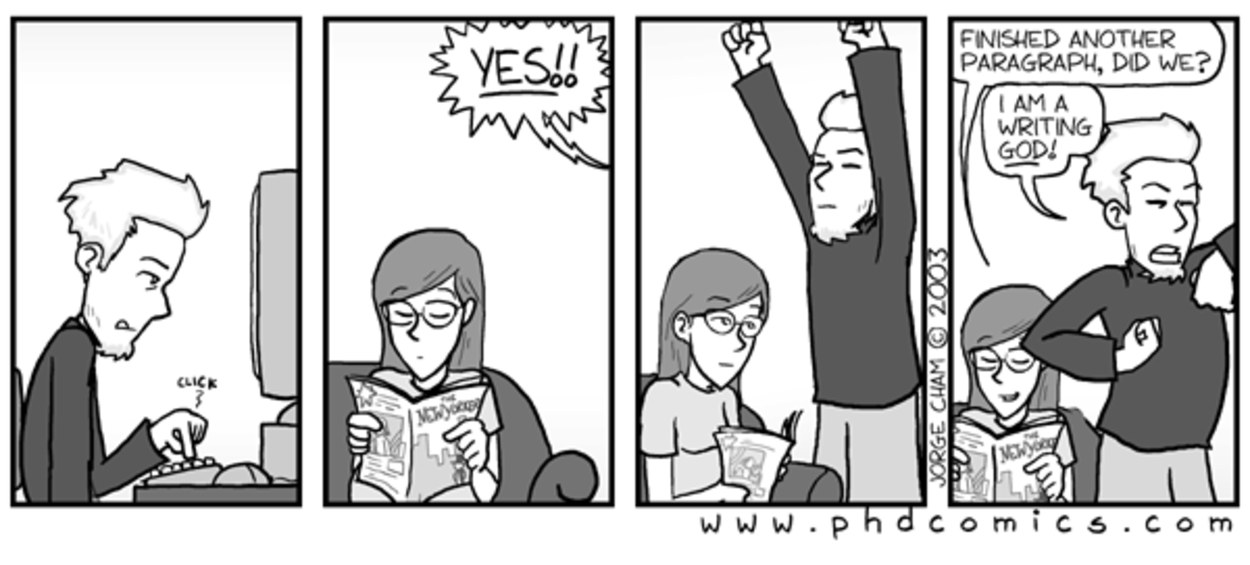
\includegraphics[width=\textwidth,keepaspectratio]{CH2/assets/comic}
\caption[Thesis Writing Comic]{A Thesis Writing Comic (from www.phdcomics.com).}
\label{fig:comic}
\end{figure}

\LaTeX{} is capable of using images in pdf, jpg and png format.

\subsection{Other Useful Commands}

There are some additional commands created to keep the formatting separated from the content, which we document below.

\keyword{keyword} -- Used to highlight keywords. For example, this is \keyword{somekeyword} (the command that produces this output is \verb|\keyword{somekeyword}|).

\keyword{tabhead} -- Used to highlight table headers. 

\keyword{code} -- Used to output code. For example, this \code{statement is formatted as code} (the command that produces this output is \verb|\code{...}|).

\keyword{file} -- Used to highlight files. For example, this is \file{somefilename} (the command that produces this output is \verb|\file{somefilename}|).

\keyword{option} -- Used to highlight options. For example, this is \option{someoption} (the command that produces this output is \verb|\option{someoption}|).

%----------------------------------------------------------------------------------------

\section{Sectioning and Subsectioning}

You should break your thesis up into nice, bite-sized sections and subsections. \LaTeX{} automatically builds a table of Contents by looking at all the \verb|\chapter{}|, \verb|\section{}|  and \verb|\subsection{}| commands you write in the source.

The Table of Contents should only list the sections to three (3) levels. A \verb|chapter{}| is level zero (0). A \verb|\section{}| is level one (1) and so a \verb|\subsection{}| is level two (2). In your thesis it is likely that you will even use a \verb|subsubsection{}|, which is level three (3). The depth to which the Table of Contents is formatted is set within \file{tmdei-style.cls}. If you need this changed, you can do it in \file{main.tex}.

%----------------------------------------------------------------------------------------

\section{In Closing}

You have reached the end of this mini-guide. You can now rename or overwrite this pdf file and begin writing your own \file{.tex} files and the rest of your thesis. The easy work of setting up the structure and framework has been taken care of for you. It's now your job to fill it out!

Good luck and have lots of fun!

\begin{flushright}
Guide written by ---\\
Sunil Patel: \url{http://www.sunilpatel.co.uk}{www.sunilpatel.co.uk}\\
Vel: \url{http://www.LaTeXTemplates.com}{LaTeXTemplates.com}
\end{flushright}

% Chapter 3

\chapter{Algorithms, Source Code, Portable Graphics and Acronyms} % Main chapter title
\label{chap:Chapter3} % For referencing the chapter elsewhere, use \ref{chap:Chapter3} 

%----------------------------------------------------------------------------------------
\section{Algorithms}

 \LaTeX{}  has several packages for typesetting algorithms in form of ''pseudocode''. In this template, we suggest the use of the \verb|algorithm| environment with the \verb|algpseudocode| package. More information about algorithms can be found at \url{https://en.wikibooks.org/wiki/LaTeX/Algorithms}.

Algorithm~\ref{alg:euclid} shows Euclid's algorithm that computes  Greatest Common Divisor (GCD) of two integer numbers.

\begin{algorithm}[b]
\caption{Euclid’s algorithm}
\label{alg:euclid}
\begin{algorithmic}[1]
\scriptsize

\State \textbf{Input}: Two integer numbers, $a$ and $b$
\State \textbf{Output}: GCD of $a$ and $b$
\State
\Procedure{Euclid}{$a,b$}\Comment{The GCD of $a$ and $b$}
\State $r\gets a\bmod b$
\While{$r\not=0$}\Comment{We have the answer if $r$ is $0$}
\State $a\gets b$
\State $b\gets r$
\State $r\gets a\bmod b$
\EndWhile
\State \textbf{return} $b$\Comment{The GCD is $b$}
\EndProcedure

\end{algorithmic}
\end{algorithm}

Here it is the \LaTeX{} text for the ''pseudocode'' algorithm presented in  Algorithm~\ref{alg:euclid}.

\begin{verbatim}
\begin{algorithm}
\caption{Euclid’s algorithm (pseudocode)}
\label{alg:euclid}
\begin{algorithmic}[1]
\scriptsize

\State \textbf{Input}: Two integer numbers, $a$ and $b$
\State \textbf{Output}:  Greatest Common Divisor (GCD) of $a$ and $b$
\State
\Procedure{euclid}{$a,b$}\Comment{The GCD of $a$ and $b$}
\State $r\gets a\bmod b$
\While{$r\not=0$}\Comment{We have the answer if $r$ is $0$}
\State $a\gets b$
\State $b\gets r$
\State $r\gets a\bmod b$
\EndWhile
\State \textbf{return} $b$\Comment{The GCD is $b$}
\EndProcedure

\end{algorithmic}
\end{algorithm}
\end{verbatim}

\verb|\listofalgorithms| command generates a list of all algorithms. This command is called in the \file{frontmatter.tex} file. Therefore, if there is no algorithm in the thesis, this command must be removed (or commented) from such file.

\section{Source Code}
Sometimes there is the need to present programming source code snippets.
The \verb|listings| package  is a powerful way to get nice source code highlighting in \LaTeX{}. It supports various programming languages, like Java (selected as the default language in this template), C, and many others.

Listing~\ref{lst:euclid_java} and Listing~\ref{lst:euclid_c} show the source code of the Euclid’s algorithm, written in Java and C, respectively.

\begin{minipage}{\linewidth}
\lstinputlisting [caption=Euclid’s algorithm (Java).,
label=lst:euclid_java]
{CH3/assets/euclid.java}
\end{minipage}

\begin{center}
\begin{minipage}{0.7\linewidth}
\lstinputlisting [language=C, 
caption=Euclid’s algorithm (C).,
label=lst:euclid_c,
numbers=none]
{CH3/assets/euclid.c}
\end{minipage}
\end{center}

Here it is the \LaTeX{} text for both listings. Note that we encapsulate the listings inside a \verb|\minipage| so that the listing does note break across pages.
Using the \verb|\lstinputlisting| command, the source code must be written in a separate file. In these two cases, both files are in \path{ CH3\assets\ } directory.

\begin{verbatim}
\begin{minipage}{\linewidth}
\lstinputlisting [caption=Euclid’s algorithm (Java).,
label=lst:euclid_java]
{CH3/assets/euclid.java}
\end{minipage}

\begin{center}
\begin{minipage}{0.7\linewidth}
\lstinputlisting [language=C, 
caption=Euclid’s algorithm (C).,
label=lst:euclid_c,
numbers=none]
{CH3/assets/euclid.c}
\end{minipage}
\end{center}

\end{verbatim}
As it can be seen from the text above, there are a lot of parameters that can be specified, like programming language (\verb|language|), numbering, etc.   
More information about listings can be found at 
\url{https://en.wikibooks.org/wiki/LaTeX/Source_Code_Listings} and 
\url{http://texdoc.net/texmf-dist/doc/latex/listings/listings.pdf}.


\verb|\listoflisting| command generates a list of all source code listings. This command is called in the \file{frontmatter.tex} file. Therefore, if there are no listings in the thesis, this command must be removed (or commented) from such file.

\section{The Portable Graphics Format}
The \gls{PGF} and a number of packages built on top of \gls{PGF} (such as TiKZ and PGFPLOTS) enable producing high quality graphical elements for your document. 
 
\subsection{TiKZ}
TikZ is built on top of PGF and allows you to create sophisticated graphics using \LaTeX{} commands. According to its author, Till Tantau~\footnote{Available online at \url{ftp://ftp.di.uminho.pt/pub/ctan/graphics/pgf/base/doc/pgfmanual.pdf}},  "\textit{What is TikZ? Basically, it just defines a number of \TeX{} commands
that draw graphics.}". With TikZ it is possible to accurately position picture elements, use \LaTeX{} fonts, incorporate mathematical typesetting, and use other \LaTeX{} features in your drawings.

The TikZ package defines the \verb|tikzpicture| environment that is required to draw a graphic. 
This environment must be inserted into a \verb|figure| environment when numbering and caption are required.
Figure~\ref{fig:tikz} shows a simple use of TiKZ, for which the \LaTeX{} source is as follows.

\begin{verbatim}
\begin{figure}[t]
\centering

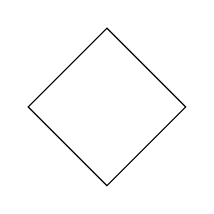
\begin{tikzpicture}
% Define four points
\coordinate (P0) at (1,0);
\coordinate (P1) at (0,1);
\coordinate (P2) at (-1,0);
\coordinate (P3) at (0,-1);
% Draw the diamond
\draw (P0)--(P1)--(P2)--(P3)--cycle;
\end{tikzpicture}

\caption{Using TiKZ for drawing pictures.}
\label{fig:tikz}
\end{figure}
\end{verbatim}

\begin{figure}[ht]
\centering

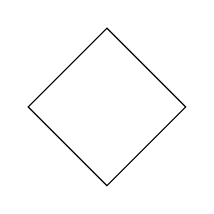
\begin{tikzpicture}
% Define four points
\coordinate (P0) at (0,0);
\coordinate (P1) at (1,0);
\coordinate (P2) at (0,1);
\coordinate (P3) at (-1,0);
\coordinate (P4) at (0,-1);
% Draw the diamond
\draw (P1)--(P2)--(P3)--(P4)--cycle;
\end{tikzpicture}

\caption{Using TiKZ for drawing pictures.}
\label{fig:tikz}
\end{figure}


A great amount of examples are available at \url{http://www.texample.net/tikz/examples/}. 
More information about TiKZ can be found at 
\url{https://en.wikibooks.org/wiki/LaTeX/PGF/TikZ} and 
\url{ftp://ftp.di.uminho.pt/pub/ctan/graphics/pgf/base/doc/pgfmanual.pdf}.

\subsection{PGFPLOTS}

PGFPLOTS provides tools to draw high quality plots, and is based on TiKZ. To use PGFPLOTS in the thesis you need to use \verb|\usepackage{pgfplots}| (in \file{main.tex}).
To guarantee compatibility you need to specify \verb|\pgfplotsset{compat=<version>}|.
You can choose the \verb|version| ().
In this case, it is recommended to choose \verb|newest|. The choice \verb|compat=newest| means "I do not care if my old figures change in appearance after the next version upgrade".

Here it is the \LaTeX{} text for create the graph presented in Figure~\ref{fig:pgfplots}.
\begin{verbatim}
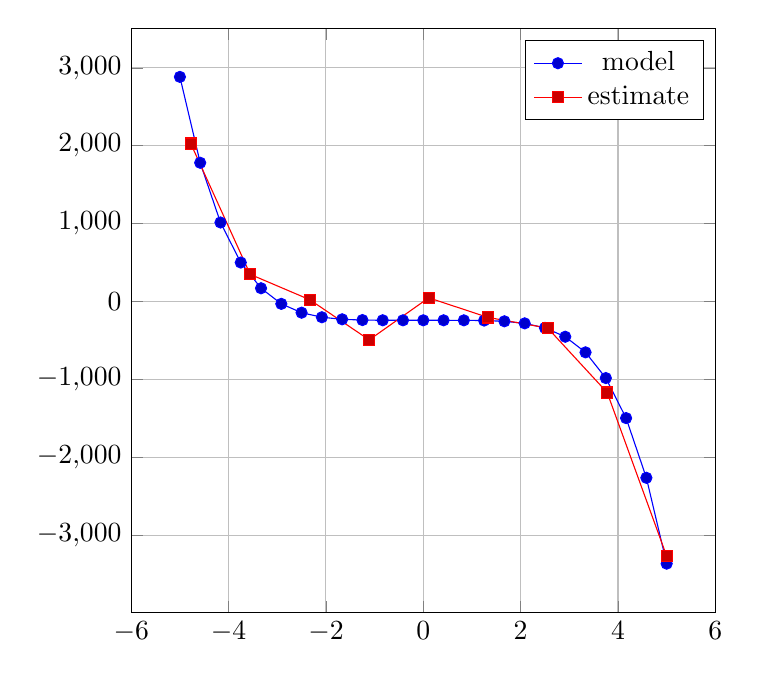
\begin{tikzpicture} 
	\begin{axis}[ height=9cm, width=9cm, grid=major, ] 
		\addplot {-x^5 - 242}; 
		\addlegendentry{model}
		\addplot coordinates { 
			(-4.77778,2027.60977) 
			(-3.55556,347.84069) 
			(-2.33333,22.58953) 
			(-1.11111,-493.50066) 
			(0.11111,46.66082) 
			(1.33333,-205.56286) 
			(2.55556,-341.40638) 
			(3.77778,-1169.24780) 
			(5.00000,-3269.56775) 
		}; 
		\addlegendentry{estimate} 
	\end{axis} 
\end{tikzpicture}
\end{verbatim}

Figure~\ref{fig:pgfplots} shows an example of a graph created using PGFPLOTS functions.

\begin{figure}[ht]
\centering
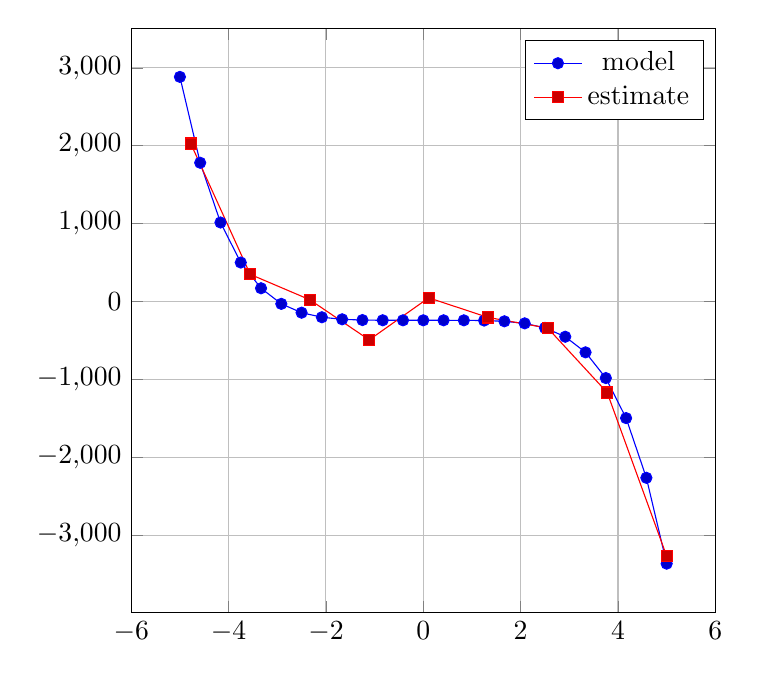
\begin{tikzpicture} 
	\begin{axis}[ height=9cm, width=9cm, grid=major, ] 
		\addplot {-x^5 - 242}; 
		\addlegendentry{model}
		\addplot coordinates { 
			(-4.77778,2027.60977) 
			(-3.55556,347.84069) 
			(-2.33333,22.58953) 
			(-1.11111,-493.50066) 
			(0.11111,46.66082) 
			(1.33333,-205.56286) 
			(2.55556,-341.40638) 
			(3.77778,-1169.24780) 
			(5.00000,-3269.56775) 
		}; 
		\addlegendentry{estimate} 
	\end{axis} 
\end{tikzpicture}
\caption{Using PGFPLOTS for drawing a graph.}
\label{fig:pgfplots}
\end{figure}

A great amount of examples are available at \url{http://pgfplots.sourceforge.net/gallery.html}. 
More information about TiKZ can be found at 
\url{http://pgfplots.sourceforge.net/pgfplots.pdf}.


\section{Handling Acronyms Automatically}
When writing a thesis you need to define acronyms.
According to Wikipedia~\footnote{Accessed in 16 of December of 2015} \textit{"An acronym is an abbreviation used as a word which is formed from the initial components in a phrase or a word."} and
\textit{"Acronyms are used most often to abbreviate names of organizations and long or frequently referenced terms."}.
Typically, an acronym is a pronounceable word, which may already exist or it can be an invented word. 

The use of acronyms imposes two rules: (i) an acronym must be defined in the text during the first appearance of the phrase or word and (ii) the document must have a list of all acronyms alphabetically sorted. In \LaTeX{} this is provided by a package called \verb|\usepackage{glossaries}| that simplifies the use of acronyms. 

Included in this thesis template there is a file called \file{glossary.tex} (in folder \file{frontmatter}), where all acronyms must be written in the form:
\begin{verbatim}
\newacronym{label}{abbrv}{full}
\end{verbatim}
where \verb|label| is the unique label identifying the acronym, \verb|abbrv| is the abbreviated form of the acronym and \verb|full| is the expanded text (word or phrase). This is an example of defining three acronyms:
\begin{verbatim}
\newacronym{RTS}{RTS}{Real-Time System}
\newacronym{GPOS}{GPOS}{General Purpose Operating System}
\newacronym{RTOS}{RTOS}{Real-Time Operating System}
\end{verbatim}

In order to use the features of the \verb|\usepackage{glossaries}|, you have only to use \verb|\gls{label}| command in the text. 
Using this command the acronym will be defined in the first appearance in the text and it will be listed in a list.
For instance, writing this \LaTeX{} text:
\begin{verbatim}
Linux is not a \gls{RTOS} but it is a \gls{GPOS}. 
VxWorks is a \gls{RTOS}, so it is not a \gls{GPOS}.
\end{verbatim}

outputs the following text: 

Linux is not a \gls{RTOS} but it is a \gls{GPOS}. VxWorks is a \gls{RTOS}, so it is not a \gls{GPOS}.

More information about acronyms can be found at 
\url{https://en.wikibooks.org/wiki/LaTeX/Glossary}.

%\input{CH4/chapter4}
%\input{CH5/chapter5}
%\input{CH6/chapter6}


%-----------------------------------------%
%--------BIBLIOGRAFIA-------------%
%-----------------------------------------%

\printbibliography[heading=bibintoc]


%-----------------------------------------%
%--------APÊNDICES-------------%
%-----------------------------------------%

\appendix % Dica para dizer ao LaTeX que os seguintes "capítulos" são apêndices

% Incluir os apêndices da tese como arquivos separados da pasta Anexos (appendices)
% Appendix A

\chapter{Appendix Title Here} % Main appendix title

\label{AppendixA} % For referencing this appendix elsewhere, use \ref{AppendixA}

As dissertações e outros trabalhos científicos podem conter apêndices ou anexos onde são expostos documentos ou outros materiais que tenham sido usados durante o trabalho, sendo imprescindível que se juntem a ele, mas que, pelo volume, não devem ser introduzidos com o texto por perturbarem a sua harmonia e lógica. São, desta forma, colocados enquanto elemento pós-textual, logo a seguir aos glossários (se existirem) ou à bibliografia. Importa, contudo, compreender o que os distingue um do outro.

Os Apêndices englobam materiais elaborados pelo autor, como conjuntos de gráficos, quadros ou tabelas de dados, eventualmente, traduções de textos, organogramas ou esquemas julgados necessários e referenciados no próprio texto.%
%\input{appendices/appendixB}
%\input{appendices/appendixC}

%----------------------------------------------------------------------------------------


%-----------------------------------------%
%--------ANEXOS-------------%
%-----------------------------------------%

% Anexos A

\chapter{Escreve o título do anexo} % Main appendix title

\label{AnnexA} % For referencing this appendix elsewhere, use \ref{AttachmentA}

Os Anexos são conjuntos de documentos não elaborados pelo autor do trabalho,
mas que serviram para a sua elaboração e facilitam a sua compreensão. Podem ser,
igualmente, tabelas, quadros, gráficos ou organogramas retirados de outros autores e
obras, mas também textos diversos ou imagens.
Os apêndices e anexos são ordenados pela letra que os designa e, cada um deles deve
começar no início de uma página ímpar (à direita).
%\input{attachments/attachmentB}
%\input{attachments/attachmentC}


\end{document}%H
